\chapter{MODEL ANALYSIS AND SELECTION\label{chapter:analysis}}

The greatest benefit researchers receive from modeling is being able to reason about the uncertainty involved in observing a phenomena of choice. From the modeling perspective, explicit statements about the uncertainty of a phenomena can be made by adding inputs to the model of the phenomena that represent a source of variance upon the phenomena.


\section{Global Sensitivity Analysis\label{sec:sens_analysis}}
A powerful tool used by modelers to quantify the uncertainty present in models is global sensitivity analysis. Broadly speaking, global sensitivity analysis is the study of how variance in the inputs of a model affect the variance, or uncertainty in the output of the model. Since the goal of the SMS pipeline is to provide modelers with a tool select a model that lowers the amount of uncertainty in estimation of a given phenomena we have chosen to use sensitivity analysis in order to evaluate the extracted models.

For this thesis we employ variance-based methods of sensitivity analysis.
% TODO: give a good definition of variational methods of sensitivity analysis
Variance-based methods of sensitivity analysis focus on the computation of sensitivity indices. Sensitivity indices are numerical values assigned to each model input, or set of inputs, that denote how sensitive the output of the model is to that input, or set of inputs. The first order sensitivity index, commonly denoted by $S1$, notates the sensitivity of the model output from each individual input. Similarly the second order sensitivity index, commonly denoted $S2$, notates the sensitivity of the model output from each pair of model inputs. This pattern continues for any given model for all higher order sensitivity indices.

The final sensitivity index is the total sensitivity index, commonly denoted as $ST$. This index has an entry that corresponds to each model input. Each entry tracks the total amount of sensitivity on the model output contributed by the input as a portion of the first, second, and all higher order sensitivity indices.

While other methods of sensitivity analysis exist, such as Variogram Analysis of Response Surfaces (VARS), the variance-based methods fit well within the scope of our problem domain as we are conducting sensitivity analysis over probabilisitic models. While the VARS method does claim a significant faster computation time, it does not reveal as information about the affects of model inputs upon the model output. This is due to the lack of pairwise-information that the variance-based methods are able to capture.

In the following subsections I will discuss three different variance-based methods of sensitivity analysis employed by the SMS pipeline.

\subsection{Sobol's Method for Index Calculation\label{sec:sobol_analysis}}
Sobol analysis is the most widely used version of variance-based sensitivity analysis. The Sobol analysis method gets its name from the sampling method used during analysis. Samples for Sobol analysis are drawn from the Sobol sequence. Defining the precise nature of the Sobol sequence is beyond the scope of this masters thesis; however, we can observe how the Sobol sequence aids sensitivity analysis by observing the differences between draws from the Sobol sequence and draws from a random sample. A visualization of the difference is shown below in figure \ref{sobol_seq_vis}.

\FloatBarrier
\begin{figure}[!htbp]
    \label{sobol_seq_vis}
    \centering
    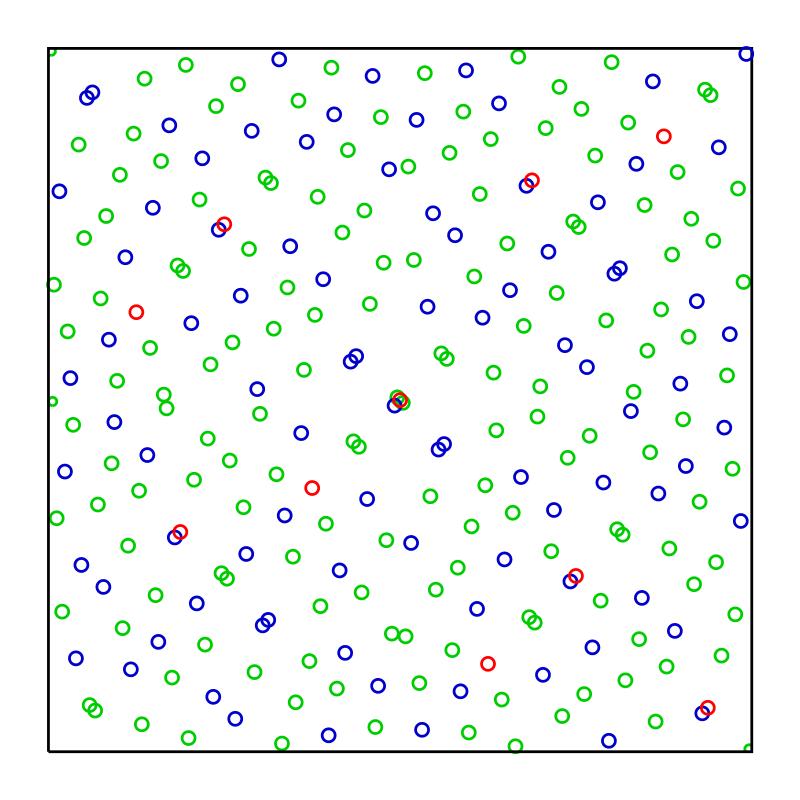
\includegraphics[width=.45\textwidth]{sobol_samples}\hfill
    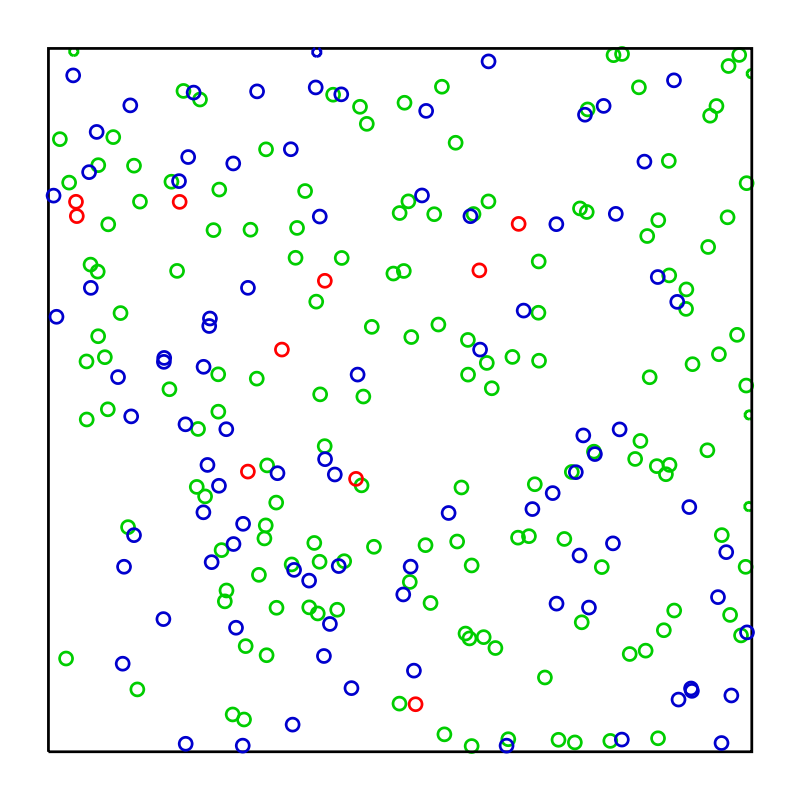
\includegraphics[width=.45\textwidth]{random_samples}
    \caption[Sobol Sequence Visualization]{A visualization of 1000 draws from the Sobol Sequence (left) paired with 1000 randomly drawn points (right) in two dimensions. For both images the first 10 draws are colored red, the remaining first 100 draws are colored blue, and the remaining 1000 draws are colored green. Images created by James Heald, distributed under a CC BY-SA 3.0 license.}
\end{figure}
\FloatBarrier

Notice that the red, blue, and green draws from the Sobol sequence are much more evenly dispersed across the sample space than the same draws from a uniform random sample. This allows the Sobol sampling method to achieve much better coverage of the search space, while still maintaining some variability in sample locations. The SMS pipeline employs a variant of the Sobol sequence introduced by Saltelli et al. that is designed to minimize the error when utilizing the samples to calculate the sensitivity indices of a function.

% TODO: maybe a little revising here
The sample matrices that must be computed for analysis are defined in algorithm \ref{sobol_sample_alg}. We can see that this sampling algorithm draws $N$ samples of $d$ dimension from the Sobol sequence and then creates $N(d+2)$ samples total to be evaluated by the model. The matrices returned from the sampling step can then be evaluated using the model computation graph. These evaluations will be represented as $f(A) \text{, } f(B) \text{, } f(\textbf{A}_{B}) \text{, and } f(\textbf{B}_{A})$. Once the evaluation step is completed, the evaluations will be analyzed according to the Sobol analyzer. The Sobol analyzer computes three different sensitivity indices using approximation equations.

\begin{algorithm}
  \caption{Sobol Sampling Algorithm}
  \label{sobol_sample_alg}
  \begin{algorithmic}[1]
    \Require $d \gets $ amount of input variables
    \Require $N \gets $ amount of desired samples
    \Require $R \gets $ set of sample space ranges for all $d$ input variables
    \State $A \gets N$ samples from $R$ using the Saltelli corrected Sobol sequence
    \State $B \gets $ shuffled rows from $A$
    \State $\textbf{A}_{B} \gets \forall i = 1 \ldots d$ $A_{B}^i = \forall j < i \; A[j] \oplus B[i] \oplus \forall j > i \; A[j]$
    \State $\textbf{B}_{A} \gets \forall i = 1 \ldots d$ $B_{A}^i = \forall j < i \; B[j] \oplus A[i] \oplus \forall j > i \; B[j]$
    \State \Return $A, B, \textbf{A}_{B}, \textbf{B}_{A}$
  \end{algorithmic}
\end{algorithm}

The $i^{\text{th}}$ element of the first order sensitivity index, $S_i$, is computed using equation \ref{sobol_s1_eqn}. Notice that this function will approximate the variance $w.r.t$ the $i^{\text{th}}$ input of the expectation $w.r.t$ all other inputs.

\begin{equation} \label{sobol_s1_eqn}
  \begin{split}
    S_i & = \frac{\mathbb{V}_{X_i}\left(\mathbb{E}_{X_{\sim i}}(Y | X_i) \right)}{\mathbb{V}(Y)} \\
     & \approx \frac{1}{N * \mathbb{V}(Y)} \sum_{j=1}^{N} f(B)_j\left( f(A_{B}^{i})_j - f(A)_j\right)
  \end{split}
\end{equation}

Once all of the first order sensitivity indices have been computed, they can be used to calculate the second order sensitivity indices. This calculation is done using equation \ref{sobol_s2_eqn} as defined below. A second order sensitivity index, $S_{ij}$, can be described as the variance of the $ij$ input pair without the variance of the separate $i^{\text{th}}$ and $j^{\text{th}}$ components.

\begin{equation} \label{sobol_s2_eqn}
  \begin{split}
    S_{ij} & = \frac{\mathbb{V}_{ij}\left(\mathbb{E}_{X_{\sim ij}}(Y | X_i X_j)\right)  - (S_i + S_j)}{\mathbb{V}(Y)} \\
     & \approx \frac{\sum_{k=1}^{N} \left(f(B_{A}^{i})_j * f(A_{B}^{k})_j\right) - \left(f(A)_j * f(B)_j\right)}{N * \mathbb{V}(Y)} - (S_i + S_j)
  \end{split}
\end{equation}

The total sensitivity indices, $S^T$, can also be calculated from the sampled matrices. The $i^{\text{th}}$ total sensitivity index can be computed using equation \ref{sobol_st_eqn} as defined below. By inspecting the result from this equation we can see that the $i^{\text{th}}$ total sensitivity index is an approximation of the expected variance caused by the $i^{\text{th}}$ input upon all other inputs $j$ such that $j\neq i$.

\begin{equation} \label{sobol_st_eqn}
  \begin{split}
    S_i^T & = \frac{\mathbb{E}_{\sim i}\left(\mathbb{V}_{X_i}(Y | X_{\sim i})\right)}{\mathbb{V}(Y)} \\
    & \approx \frac{1}{2N * \mathbb{V}(Y)} \sum_{j=1}^{N} \left(f(A)_j - f(A_{B}^{i})_j\right)^2
  \end{split}
\end{equation}

\subsection{FAST S1 Index Calculation\label{sec:fast_analysis}}
Some text.

\subsection{RBD-FAST S1 Index Calculation\label{sec:rbd_fast_analysis}}
The purpose of utilizing the RBD-FAST method of sensitivity analysis is to further lower the runtime of analysis as compared to the standard FAST method. It has been claimed that RBD-FAST can lower the runtime of sensitivity analysis for models with a large number of input parameters.

\section{Model Output Surface\label{sec:out_surf}}
A Model Output Surface (MOS) plot is a 3D plot where the z-axis is the output variable of a model and the remaining axes are input variables. A MOS plot consists of the plotted outputs over a predefined range for each of the two inputs which creates a smooth surface object in three dimensions. Evaluation to create this surface is done using a mesh grid of finite points. extrapolation between point evaluations can then be conducted to create the smooth surface visualization. As expected, a higher number of input samples over the same input space range will lead to a smoother surface that is a more accurate representation of the true output surface for the input pair. In this section I will cover the process of selecting which input variables to study with MOS plots, how to set values for the additional inputs not under study, and how to efficiently perform the evaluations necessary to generate a MOS plot.

\subsection{Input Variable Selection\label{sec:inp_var_sel}}
Most models will have more than two input variables and thus when creating a MOS plot a decision must be made about which two input variables should be varied during output surface creation. Generally speaking, for a model with $N$ input variables, a user could generate $\frac{N(N+1)}{2}$ plots to expose all possible pairs of variable interactions and examine how those interactions affect the output surface. For most sizes of $N$ this study is likely to not be computationally feasible, and modelers are unlikely to desire to view such a large number of output plots when performing model selection. A better use-case for MOS plots would be to showcase the pairs of variables that have the greatest combined affect on the model output.

In order to accomplish this task we need a way to rank the pairs of inputs in order of how greatly they affect model output. Fortunately we can attain this ranking directly from the second order sensitivity index, $S2$. Utilizing the $S2$ index as our ranking schema we can either create MOS plots for the top $k$ variable pairs, or we can use a threshold cutoff and create MOS plots for all pairs on input variables that exceed this cutoff. An appropriate cutoff could be a pre-defined value, or it could be based upon a difference between neighboring values of the sorted $S2$ indices. An example of such a cutoff would be to generate MOS plots for all input pairs, until seeing a drop in $S2$ index score of at least an order of magnitude.

It is important to note that utilizing the $S2$ index is not the only way to select which input pairs to generate a MOS plot for, and is likely not the only metric of interest to modelers. If we have additional information, such as which inputs can be most or least accurately measured by the modelers then we may want to generate MOS plots for the modelers based upon this criterion so they can observe how output varies for input variables that they can measure well, vs those that they can measure poorly. This will become even more important for the task of model selection when competing models have differing sets of inputs, some of which may be easier or harder to measure than others.

\subsection{Input parameter estimation\label{sec:inp_param_est}}
Once the input variables for a given MOS plot are selected, the remaining inputs must have values assigned to them to allow for the model to be evaluated for MOS plot generation. To avoid confusion, I will refer to this set of input variables that will no longer be varied as the input parameters for the model.

There are many options present for assigning values to each of the input parameters. Unfortunately the nature of models also demands that either one or few values be chosen for each of the input parameters due to the high number of input parameters that are likely to be present. Even if we wished to allow for only two values for each input parameter, and wanted to study all possible combinations of them then for a set of $N$ input parameters we would generate $2^N$ MOS plots. Expecting modelers to review this many MOS plots goes against the idea of summarizing model behavior. This entails that a single set of values for the input parameters should be selected.

The task of input parameter estimation is now the task of finding the best-fit set of input parameters for a MOS plot. For each parameter we know that we have a range of values that were used for the parameter during analysis. From this information we can define that the best-fit for an input parameter is the Maximum Likelihood Estimate (MLE) over the range. The MLE is a useful estimate for each input parameter since the ranges are included for each parameter. However, if observational data were present, then it would be possible to use the Maximum A Priori (MAP) estimate as the setting for our input parameters.

% \subsection{Surface Generation and Evaluation\label{sec:surf_usage}}
% Some text.

\section{Model report generation\label{sec:report_gen}}
Some text

\subsection{Comparative Sensitivity Index Assessment\label{sec:comp_sens_ind}}
Some text.

\subsection{Cross-model Sensitivity Surface Examination \label{sec:multi_mod_surface}}
Some text.
